\chapter{Mathematische Grundlagen}
F\"ur die Bildverarbeitung werden eine Reihe mathematischer Methoden ben\"otigt. In diesem Kapitel werden alle notwendigen mathematischen Grundlagen kurz vorgestellt und erl\"autert.

\section{projektive Geometrie}
Die Mathematik stellt verschiedene algebraische Repr\"asentationen von geometrischen Objekten und Transformationen, auch Geometrien genannt, zur Verf\"ugung.\cite{Schindler2015} Klassischerweise wird die euklidische Geometrie verwendet um die Umgebung zu beschreiben. Diese bietet, aufgrund des Vorhandenseins von Gr\"o{\ss}en wie beispielsweise L\"angen und Winkeln, eine Beschreibungsweise, die auch unserer Vorstellung des Raumes entspricht.
In der euklidischen Geometrie werden Punkte in einer zweidimensionalen Ebene oder im dreidimensionalen Raum durch zwei- beziehungsweise dreidimensionale Vektoren, sogenannte inhomogene Koordinaten, dargestellt. F\"ur Punkte, im euklidischen Raum, werden zwei m\"ogliche Transformationen definiert: die Rotation und Translation. Au�erdem liegt eine \"Aquivalenz zweier Punkte nur dann vor, wenn die Koordinaten beider Punkte identisch sind.\cite{Rahmann2011} 
Betrachtet man nun, aus der Sicht eines Menschen oder einer Kamera, ein Paar paralleler Linien, so wird man feststellen, dass die Linien in einem Fluchtpunkt zusammenlaufen. Ebenso weist ein Objekt, welches aus rechtwinkligen Strukturen aufgebaut ist, das Ph\"anomen der perspektivischen Verzerrung auf. Die Verzerrung bewirkt, dass die ehemals rechten Winkel auf Winkel ungleich $90$ Grad abgebildet werden. Diese Sonderrolle, welche die parallelen Geraden in der euklidischen Geometrie einnehmen, wird in der projektiven Geometrie aufgehoben\cite{Wahner2011}. Die projektive Geometrie erweitert die euklidische Geometrie, um Punkte im Unendlichen, sogenannte Fernelemente. Diese Fernpunkte dienen als Schnittpunkte f\"ur Scharen paralleler Geraden und geben die Richtung der Geraden an. \cite{Wahner2011}

\subsection{Der projektive Raum}
\begin{figure}[htb]
\centering
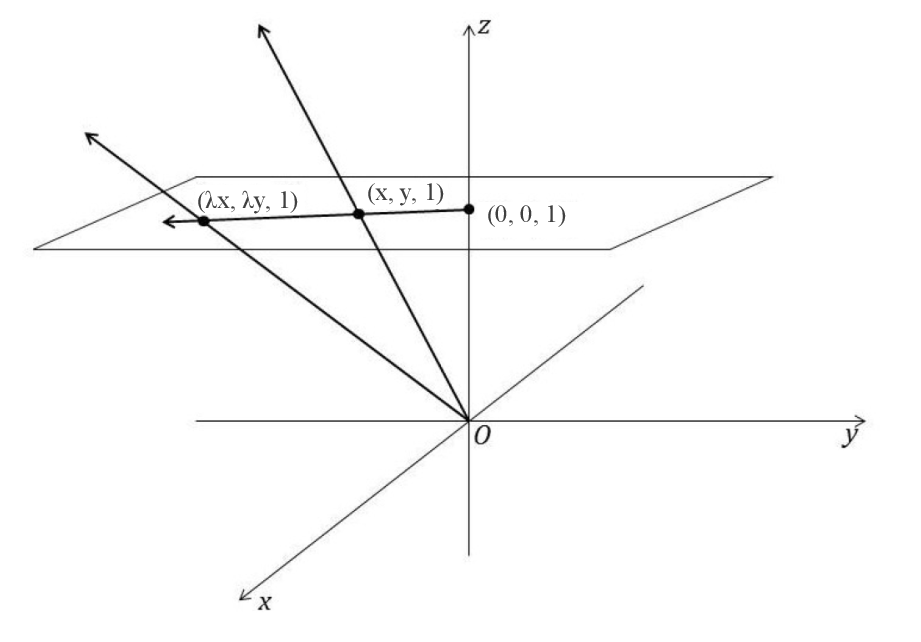
\includegraphics[width=0.8\textwidth]{proGeo_lambda.png}
\caption{die projektive Ebene ${\mathbb{P}}^{2}$ kann als eine eingebettete Ebene im ${\mathbb{R}}^{3}$ verstanden werden \cite{Wahner2011}} 
\label{fig:progeo}
\end{figure} 
Anschaulich werden die Fernpunkte, wenn man eine Ebene betrachtet, die in dem dreidimensionalen Raum ${\mathbb{R}}^{3}$ eingebettet ist. Die Ebene liege parallel zur \textit{xy}-Ebene bei $z = 1$, siehe Abbildung \ref{fig:progeo}. Weiterhin gilt allgemein, dass es f�r jeden Punkt auf der Ebene eine Gerade gibt, die die Ebene schneidet und durch den Ursprung geht. Damit l\"asst sich jedem Punkt der Ebene ein Richtungsvektor zuordnen. Dieser Richtungsvektor kann beispielsweise der Punkt $(x,y,1)$ selbst oder ein skalares Vielfaches von ihm $(\lambda x,\lambda y,1)$, mit $t \in \textbf{R} \setminus \{0\}$, sein. 
Ein beliebiger Punkt auf der Ebene $(\lambda x,\lambda y,1)$ kann ebenfalls als $(x,y,\frac{1}{\lambda})$ geschrieben werden. Man sieht, dass sich der Punkt f�r $\lambda \to \infty$ vom Ursprung entfernt und zu einem Fernpunkt mit $(x,y,0)$ wird. Fernpunkte repr\"asentieren damit die Richtung eines Geradenb�schels\cite{Wahner2011}. Allgemein werden endliche Punkte durch Vektoren der Form $(x,y,1)$ und unendliche Punkte durch $(x,y,0)$ dargestellt.

\subsection {Euklidische und projektive Koordinaten}
Im \textbf{n}-dimensionalen euklidischen Raum ${\mathbb{R}}^{n}$ wird ein Punkt durch einen n-dimensionalen Vektor $\textbf{x} = (x_1,\dots ,x_n)^T$ beschrieben. Diese Darstellung wird auch inhomogene Koordinaten genannt.\\
Ein Punkt im n-dimensionalen projektiven Raum ${\mathbb{P}}^{n}$ wird durch einen \textbf{(n + 1)}-dimensionalen Vektor $\textbf{\~x} = (x_1,\dots ,x_{n+1})^T$ dargestellt. Man spricht in diesem Fall von homogenen Koordinaten. Der Nullvektor $\textbf{0}_{n+1}$ ist kein Element vom ${\mathbb{P}}^{n}$, da er keiner geometrischen Gr\"o{\ss}e im projektiven Raum entspricht. Die \"Uberf\"uhrung von euklidischen Koordinaten in projektive Koordinaten l\"asst sich einfach mit folgender Beziehung durchf\"uhren.
\begin{equation}
	(x_1, \dots, x_n) = \textbf{x}\rightarrow \textsl{\~x}= (\lambda x_1, \dots,\lambda x_n, \lambda) 
\end{equation}
Dabei ist $\lambda$ ein beliebiger Skalierungsfaktor, mit $\lambda \in \textbf{R} \setminus \{0\}$. Durch die Betrachtung der R\"uckkonvertierung wird ersichtlich, warum es notwendig ist die Null auszuschlie{\ss}en.
\begin{equation}
	(x_1,\dots,x_n,x_{n+1}) = \textsl{\~x} \rightarrow \textbf{x} = (\frac{x_1}{x_{n+1}},\dots,\frac{x_n}{x_{n+1}})
\end{equation}
Aus dieser Konvertierung ergibt sich auch, dass die \"Aquivalenz zweier projektiver Punkte die Gleichheit der homogenen Koordinaten, bis auf einen Skalierungsfaktor, bedeutet. Daher spricht man bei homogenen Koordinaten auch von Verh\"altniskoordinaten. Punkte der Form $\textsl{\~x}_{\infty}= (x_1,\dots,x_n,0)^T$ sind Punkte im Unendlichen und werden ideale Punkte genannt. Ideale Punkte k\"onnen offensichtlich nicht in inhomogene Koordinaten \"uberf\"uhrt werden. Damit bildet der euklidische Raum einen Teilraum des projektiven Raums\cite{Rahmann2011}.

\subsection{Transformationen}
Im projektiven Raum sind eine Reihe von Transformationen definiert. Da f\"ur die Kalibrierung die Betrachtung der projektiven Ebene ausreicht, wird nur diese behandelt. Alle behandelten Eigenschaften gelten allerdings auch f\"ur den projektiven Raum. Die Transformationen bilden eine Hierarchie. Die allgemeinste Transformation ist die projektive Transformation, darauf folgt die affine Transformation, die \"ahnliche Transformation und die euklidische Transformation, welche die speziellste Transformation ist. F\"ur jede Gruppe von Transformationen gibt es sogenannte Invarianten\footnote{geometrische Gr\"o�en, die durch die Transformation nicht ver\"andert werden}. Die Anzahl von Invarianten nimmt mit der Spezialisierung der Transformation zu. Dabei ist jede Invariante der Obergruppe auch gleichzeitig eine Invariante jeder abgeleiteten Untergruppe \cite{Rahmann2011}.

\subsubsection{projektive Transformation}

Die projektive Transformation ist die allgemeinste Transformation. Sie bildet Punkte auf Punkte und Linien auf Linien ab. Die Beschreibung der projektiven Transformation ist mit Gleichung \ref{eq:proTrans} m\"oglich.
\begin{equation}
\text{\~{x}' }\thicksim \textbf{H} \text{\~{x}}
\label{eq:proTrans}
\end{equation}
Dabei ist \textbf{H} eine regul\"are $3x3$ Matrix. Weiterhin sei die Gleichung homogen. Die Abbildung wird Homographie genannt. Aus der Eigenschaft der regul\"aren Matrix l\"asst sich die Invertierbarkeit der Transformation ableiten. Da es sich um eine homogene Gleichung handelt, sind alle Matrizen \textbf{H} \"aquivalent, so lange sie sich nur durch einen Skalierungsfaktor unterscheiden. Die einzige Invariante der projektiven Transformation ist das Doppelverh\"altnis: $\frac{|AB||CD|}{|AC||BD|}$, wobei A,B,C und D Punkte auf einer Geraden sind und $|AB|$ der Abstand zwischen zwei Punkten ist. Bei neun Matrixelementen ergeben sich acht Freiheitsgrade, da der Skalierungsfaktor abgezogen werden muss \cite{Rahmann2011}. Die projektive Transformation erlaubt die Abbildung unendlich weit entfernter Punkte auf endlich weit entfernte Punkte.
\subsubsection{euklidische Transformation}
Wie bereits erw\"ahnt, ist die euklidische Transformation(Gleichung \ref{eq:euklidTrafo}) die spezialisierteste Transformation im projektiven Raum. 
\begin{equation}
\text{\~{x}' }\thicksim \textbf{H}_\textbf{S} \text{\~{x}}
 = 
\begin{pmatrix}
\textbf{R} & \textbf{t} \\
\textbf{0}^T & 1 \\
\end{pmatrix}
\text{\~{x}}
\label{eq:euklidTrafo}
\end{equation}
Sie ist durch eine Rotation und eine Translation beschrieben und besitzt als Invarianten L�ngen und Fl�chen\cite{Rahmann2011}. \textbf{R} ist eine  Rotationsmatrix und \textbf{t} der Translationsvektor. F\"ur den ${\mathbb{R}}^{2}$ gilt:
\begin{equation}
\textbf{H}_\textbf{S}
 = 
\begin{pmatrix}
cos(\alpha) & -sin(\alpha) & x \\
sin(\alpha) & cos(\alpha) & y \\
0 & 0  & 1 \\
\end{pmatrix}
\label{eq:Hs}
\end{equation} 

\subsubsection{Inverse Perspective Mapping}\label{sec:IPM}
Unter dem sogenannten \textit{inverse perspective mapping}(IPM) versteht man eine geometrische Transformation, die die Effekte der perspektivischen Projektion umkehrt. Daf\"ur wird das Bild in die Vogelperspektive transformiert. 
\begin{figure}[ht]
\centering
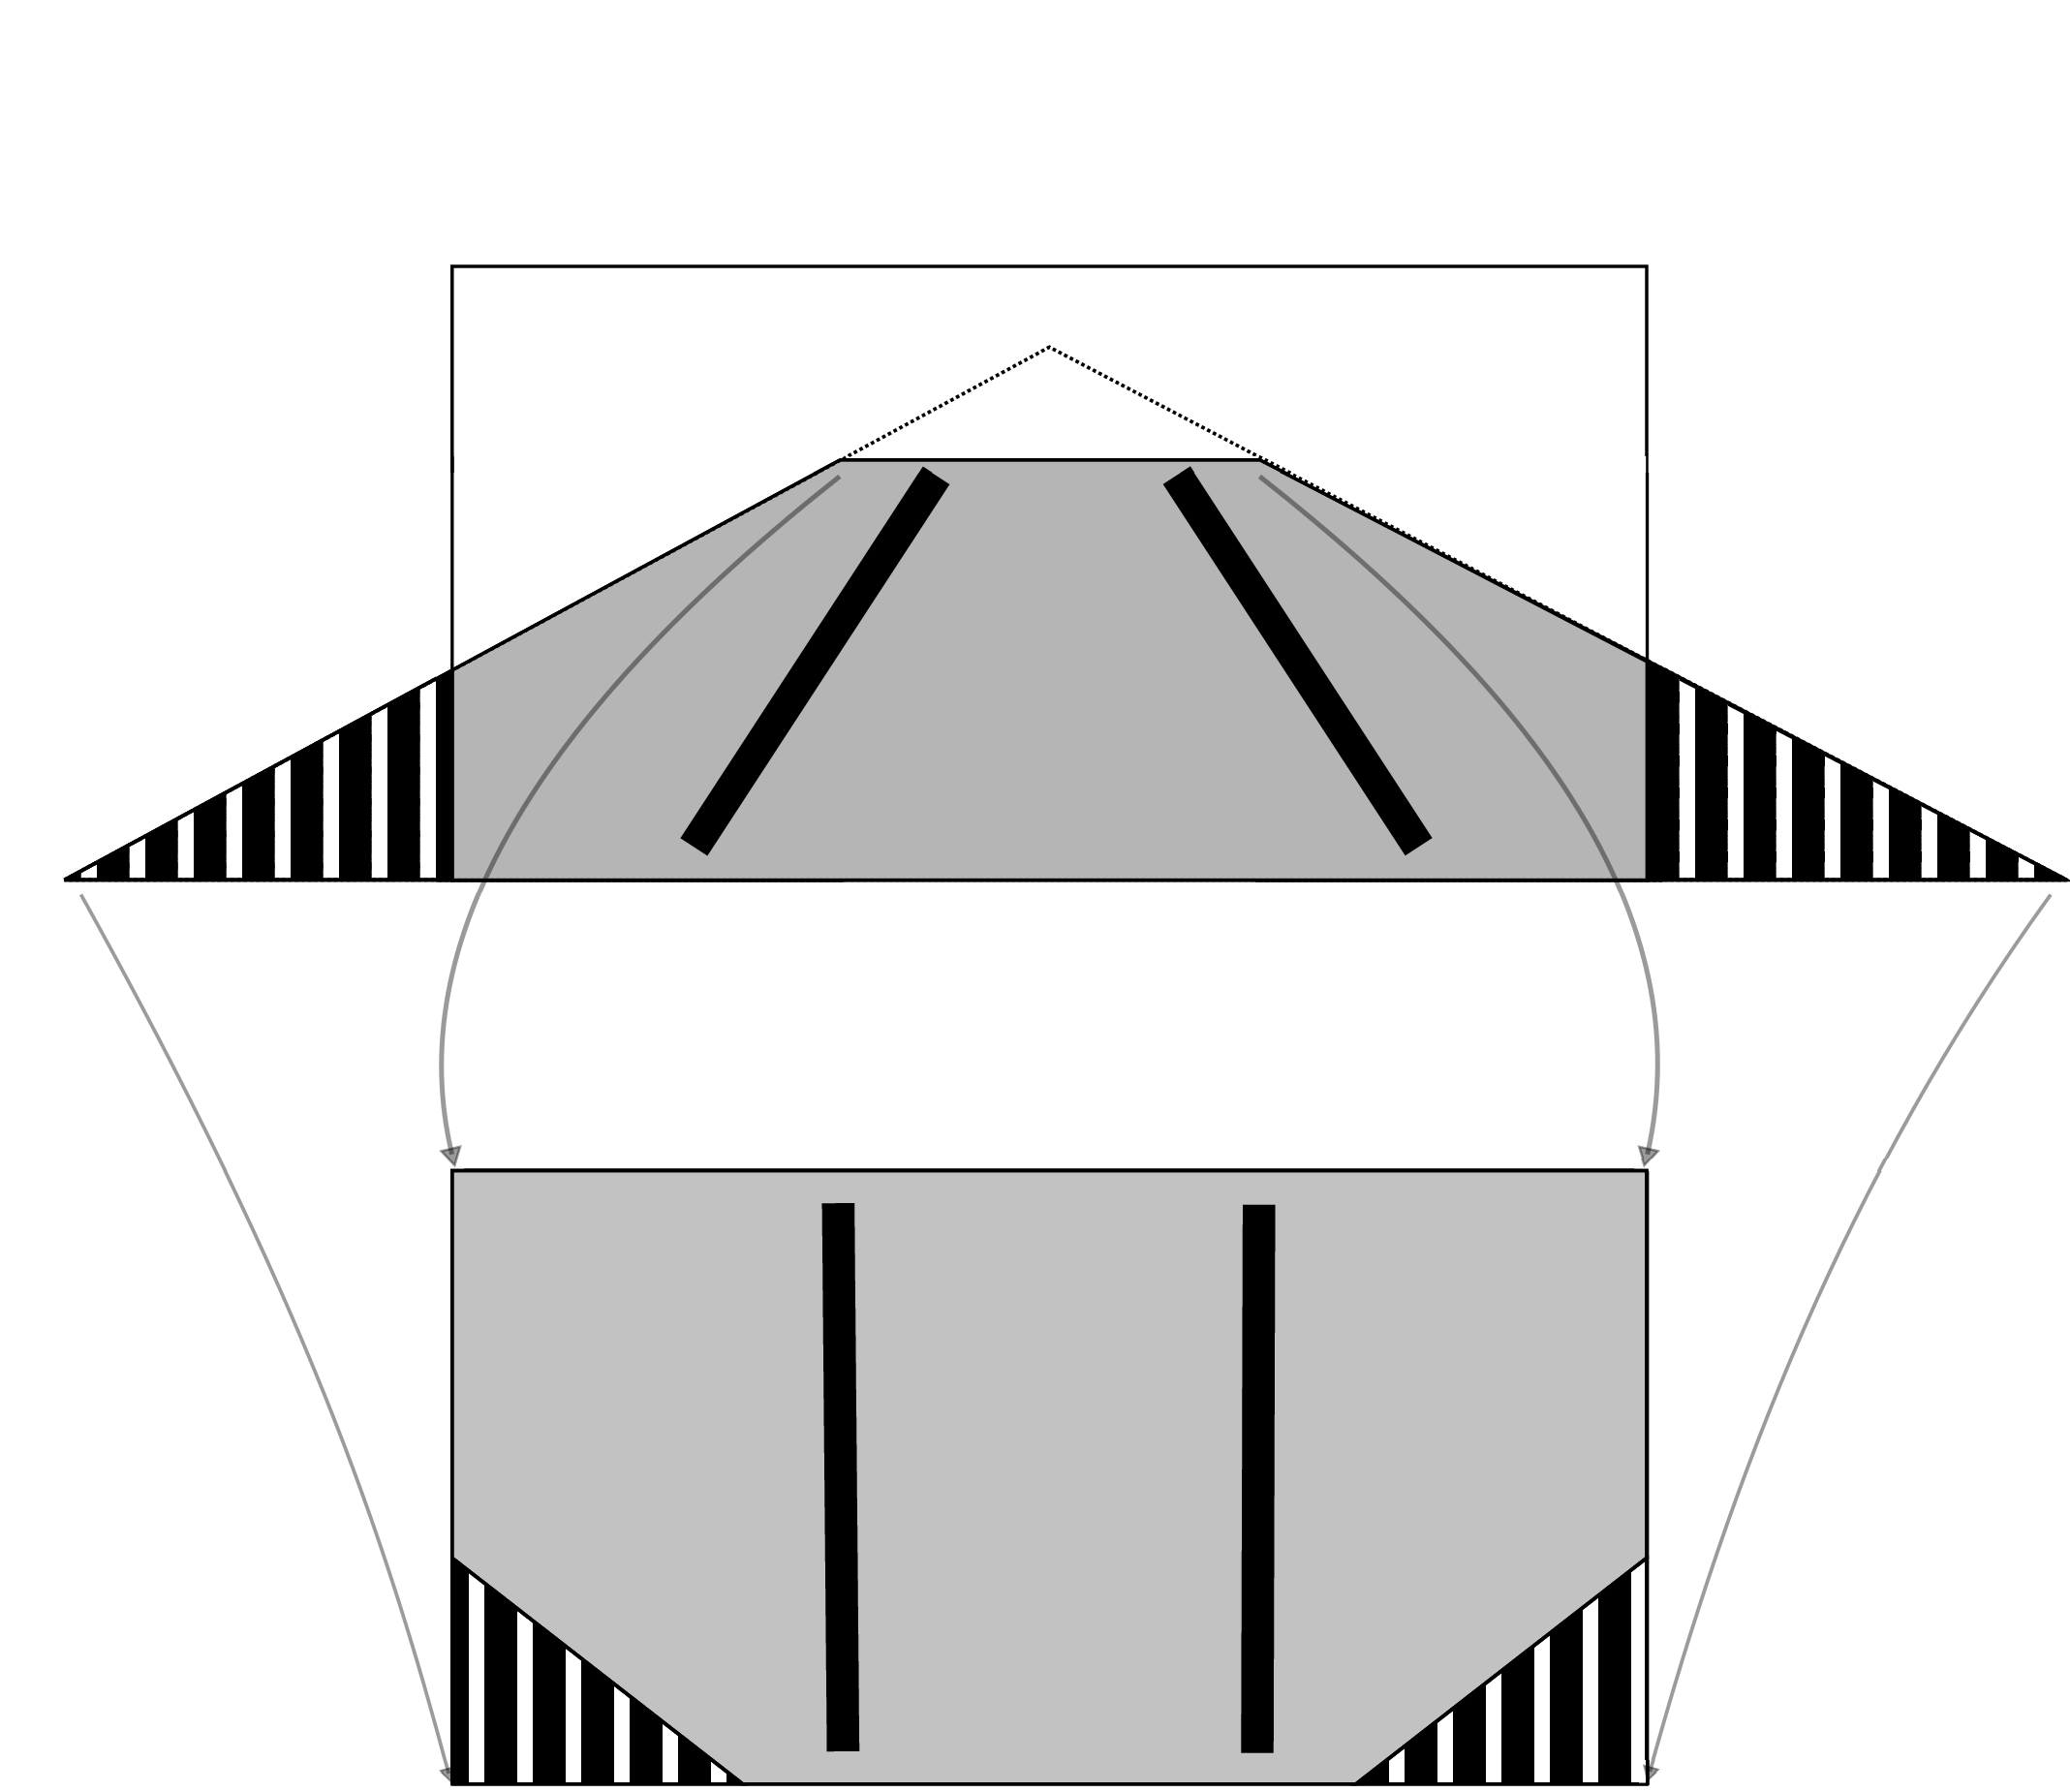
\includegraphics[width=0.8\textwidth]{IPM_Prinzip.png}
\caption{Bei der inversen perspektivischen Transformation werden die Punkte des Ausgangsbildes auf andere Koordinaten abgebildet. Hier dargestellt: die Transformation in die Vogelperspektive} 
\label{fig:IPM_Prinzip}
\end{figure} Abbildung \ref{fig:IPM_Prinzip} zeigt die prinzipielle Funktionsweise der Transformation. Es wird ein Ausschnitt des urspr\"unglichen Bildes auf ein neues Bild abgebildet \cite{AMM2004}. Die Durchf\"uhrung der Transformation ist durch zwei unterschiedliche Verfahren m\"oglich. Die erste berechnet f\"ur jedes Bild eine neue Homographie. Damit ist es beispielsweise m\"oglich, die Transformation auch dann durchzuf\"uhren, wenn die Fahrbahn eine Steigung besitzt. Allerdings ist dieses Verfahren mit hohem Rechenaufwand verbunden. Eine schnellere Methode ist das sogenannte Remapping. Daf\"ur muss im Initialisierungsschritt einmalig eine Punktkorrespondenz gefunden werden, die die Transformation durchf\"uhrt. Mit den Korrespondenzen werden f\"ur das Eingangs- und Ausgangsbild jeweils eine sogenannte \textit{Map} erzeugt. Die \textit{Maps} speichern, auf welche Punkte im Ausgangsbild die Punkte vom Eingangsbild abgebildet werden. Im sp\"ateren Betrieb muss das neue Bild nur einem \textit{remapping} - Schritt unterzogen werden. Dabei werden die Pixel, auf Grundlage der erstellen \textit{Maps}, neu angeordnet. Der Nachteil dieser statischen Methode ist, dass, beispielsweise eine Fahrbahn mit Steigung, nicht korrekt in die Vogelperspektive transformiert wird.
